% used for market drawings
\newlength{\slotwidth}
\setlength{\slotwidth}{.103\textwidth}

\section{Markets for a Self-Incentivizing Network}
\label{sec:designs}
Our goals for a market were as follows:
\begin{itemize}
\item Let anyone contribute capacity
\item Allow users to selfishly maximize their own utility functions
\item Allow users to buy guarantees of packet carriage
\item Allow users to adapt to changes in demand? TODO reword or remove
\end{itemize}
A market could be exposed by a single router or a gateway connected to multiple network capacity providers.
We envision users could also interact with multiple markets.

In following section, we sketch a simple market we designed to achieve these goals and then evaluate its performance with simulated users.
We outline our current performance as well as the limitations of our market and them propse a multiresolution market that addresses the issues we found.
%Our intial design has high overhead and our current simulated users have the ability to change their utility for the worse because of market races with other users. We quantify this phenomena with a worst case \emph{evil user}, and finally propose a new multi-resolution market that addresses these problems.

\subsection{Simple Market Design}
Our market is composed of consecutive time slots in which a packets can be delivered. Users are able to buy the rights to send a packet at a given time slot.
Once a slot is owned by a user, they have a guaruntee their packet will be carried to its next destination at that time if they can deliver it to the router before that time. Users who own a slot can also post an offer to re-sell their slot to another user for a given price.
%With this mechanism, users can be granted guaruntees of packet carriage but also change to increase their own percieved utility.
Figure \ref{f:simple_market} gives an example of the basic market state.

\begin{figure*}
\renewcommand{\arraystretch}{2}
\begin{tabular}[height=3in]{|*{8}{p{\slotwidth}|}}
\hline
Time: 0 & Time: 1 & Time: 2 & Time: 3 & Time: 4 & Time: 5 & Time: 6 & Time: 7 \\
\{(A, \$2.01)\} & \{(A, \$2.01)\} & \{(B, )\} & \{(B, )\} & \{(ISP, \$1)\} & \{(ISP, \$1)\} & \{(C, \$10)\} & \{(ISP, \$1)\} \\
\hline
\end{tabular}
\caption{Simple market sample state. User A owns the first two time slots and has an offer of \$2.01 for each. User B owns the next two slots and has not put up an offer to sell them. User C owns slot at time 6 and has posted an offer of \$10 to sell it. ISP owns remaining slots with an offer of \$1 for each.}
\label{f:simple_market}
\end{figure*}

\subsection{User types}
The objectives of market users could vary greatly. Four example user types are outlined in Figure~\ref{f:user_types}, and many more are possible.
\begin{figure*}
\begin{tabular}{|p{.25\textwidth}|p{.70\textwidth}|}
\hline
User Type & Objective \\
\hline
\hline
Flow completion time user & Send $n$ minimizing flow completion time \\
\hline
Consistent bandwidth user & Send $n$ packets every $t$ milliseconds. Example values $t=100$ for interactive audio/video or $t=$ current buffered time for video streaming \\
\hline
Deadline user & Send $n$ packets by deadline $d$. $d$ could be a few seconds for an email message to many hours for a low cost data backup.\\
\hline
Evil user & Maximally reduce utility of another market user while staying within a budget $c$ \\
\hline
Capacity owner user & Add capacity slots market at reserve price \$$r$\\
\hline
\end{tabular}
\caption{Example types of users}
\label{f:user_types}
\end{figure*}

\subsection{Implementation}
\subsubsection{Market Simulator}
The market simulator takes a set of user bots and runs them in round robin order giving them the current order book, packets sent, and money exchanged. The simulator runs until all users have stopped changing the order book, then advances time by declaring the front-most packet on the order book sent. This process is repeated until all flows have completed. We this this model is sufficiently realistic to simulate a home router that would push the order book to interested machines when it changed.

\subsubsection{Flow completion time user bot}
We implemented a flow completion time user bot for the simulator which arrives at a set time and has a set number of packets $n$ it would like to send as soon as possible. It tries to maximize the utility function $U= -d - c$, where $d$ is the total flow duration and $c$ is the total amount paid for slots.
Upon arrival, this user buys the $n$ slots that maximize its utility function. Once slots have been purchased, it puts up an offer for each slot it owns priced at \$.01 more than negated loss of utility the user would experience if it did not own that slot and had to buy another one.

\subsection{Simple Market Evaluation}
\begin{figure}
%\vspace{\baselineskip}
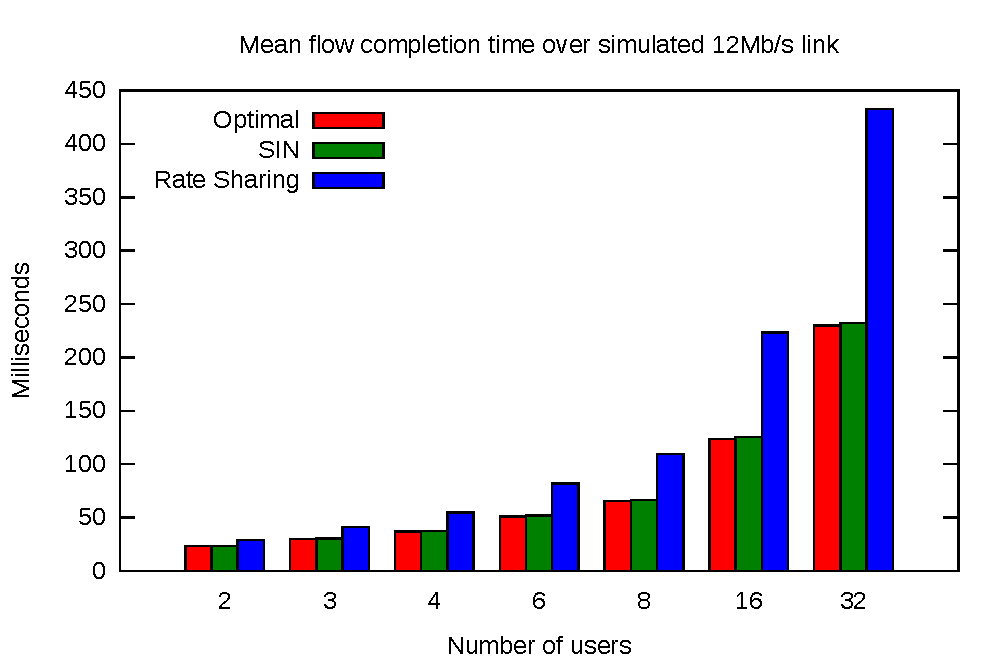
\includegraphics[width=\columnwidth]{plots/delay_over_srtf.pdf}
\caption{Simulation results for 32,000 flows with varying concurrency.}
\label{f:delay_over_srtf}
\end{figure}

\begin{figure}
%\vspace{\baselineskip}
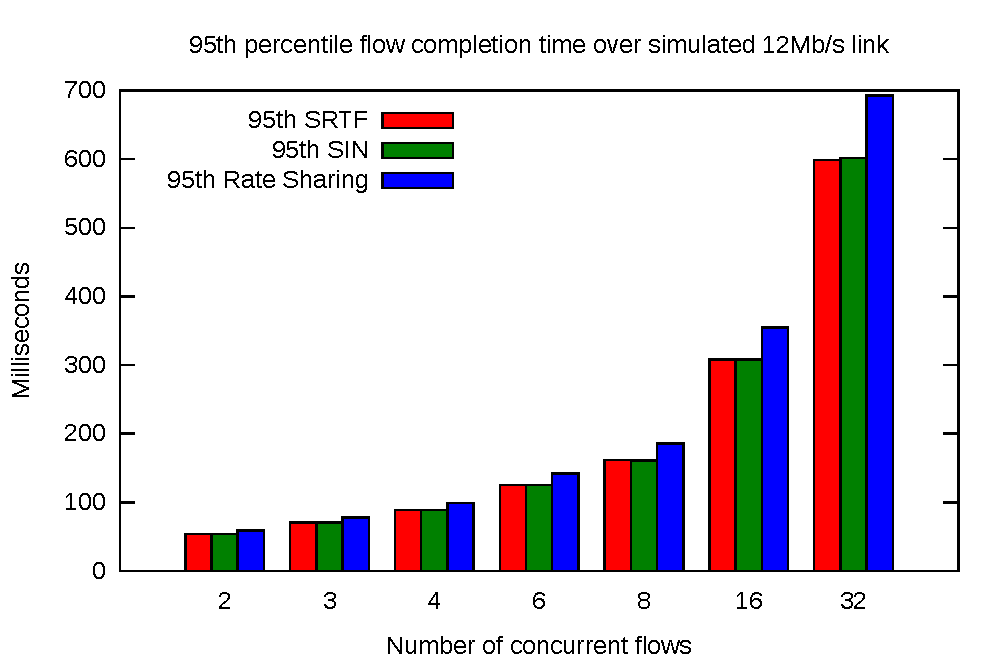
\includegraphics[width=\columnwidth]{plots/95th_delay_over_srtf.pdf}
\caption{95th percentile flow duration.}
\label{f:95th_delay_over_srtf}
\end{figure}

We simulated the results of running a market in practice with flow completion time users that would arrive at time $t$ had a known number of packets $n$ they wanted to send.
Figures~\ref{f:delay_over_srtf} and \ref{f:95th_delay_over_srtf} show the result of running the simulation with 2 to 32 concurrent flow completion time user bots. In this simulation flows arrive at time $uniform(0, 39)$ and have length $uniform(1, 40)$ MTU size packets.
The link being scheduled can send one MTU packet per millisecond (12Mb/s). In the market case, this is manifested by a single owner user that provides 1 packet of capacity every millisecond with an initial offer of \$1 per slot.

We compare the mean flow duration achieved by our market against the shortest remaining time first schedule and an equal rate sharing or round robin schedule. Shortest remaining time first (or SRTF) achieves the minimum possible mean flow duration for an online algorithm with known job durations\cite{karger10,bansal01} (SRTF is also called shortest remaining processing time in some literature).
Rate sharing is an idealized model of what TCP would achieve on FIFO queued router with a large buffer.

As our figures show, the selfish acting bots in our market simulation always converge on a near optimal flow mean flow duration schedule for the link. The majority of time wiht a smaller number of concurrent users, the schedule produced by the market was equivalent to the SRTF schedule. For all numbers of users, the market schedule had mean flow duration that was less than 1\% higher than SRTF.
TODO: talk about 95th chart

\subsubsection{Market Benefits}
SRTF minimizes the mean flow duration but does not attempt to be fair to users. For example, a string of short flows will starve a long flow \cite{bender98}.
Our market recovers solutions equal or close to SRTF in terms of mean flow duration, but it also more fairly distributes value among its users.
If a new flow arrives to a busy market, it must either wait to go after existing flows or directly compensate the owners of the flows it preempts. Like SRTF, a long flow in our market could be starved indefinately by the repeated arrival of short flows, however, this starvation is voluntary by the owner who puts offers up and they would be compensated to infinity to do so.

TODO: it would be cool to have a graph of user utility
\subsubsection{Market Incentives}
Someone who contributes network capacity to the market would be compensated based on the prices they set.
In our current scheme, the market is acting in the interest of its users in sharing the order book and facilitating trades between users.
To incentivize the market to function efficiently, the market could potentially tax every transaction made through it. We will leave further analysis down this path for future work.

\subsubsection{User Disappointment}
Unfortunately, in simulation it is possible that a user bot would have had a higher utility at the end if it refused to put offers on slots it had purchased.
This is possible because our flow completion time user bot bases its offer prices on the offer prices of the slots they would buy instead if their slots are sold, but they are not always able to purchase those replacement slots for those prices (for example if they were sold to someone else who raised the price).
In an attempt to avoid this, users frequently re-price their slots, but unless their price can instantly reflect a price change, this possibility of a user hurting their final utility is unavoidable with our current market.
%replacement slot, but if cost of that replacement slot goes up that slot can be purchased and their offer can be matched before they can re-price their offer.

We call this phenomena \emph{disappointment} beause a user puts offers on slots it owns expecting to only increase their overall utility function in the future but instead have it reduced. User dissapointment could potentially lead to users putting higher offers or no offers at all on slots they own, which would reduce the quality of schedules the market produces.
The user disappointment problem has parallels to the \emph{exposure problem} of auction theory \cite{milgrom00, englmaier06} because the slot prices are dependent on each other.
%While user disappointment does happen sometimes in our simulations (TODO maybe figure for this), a user normally increases their utility when they list a slot.
Disappointment can be arbitrarily bad in the case of a hypothesized evil user: whose sole objective is to reduce the utility of another user.
\subsubsection{Evil User}
An evil user could maximally reduce the utility of a flow completion time user for the cheapest cost by buying the cheapest slot that that user has for sale, and then buying the next $m$ slots after the last packet of the flow completion time user without putting up offers for any slots. Unless the flow completion time can move earlier, this reduces the utility function of the flow completion time user by $m$.%(TODO need example with reserve prices I think. Possbily diagram.)
% talk about how this still better than current situation because evil user has to pay?, lots of faith in current implementations
\subsubsection{Communication overhead}

\begin{figure}
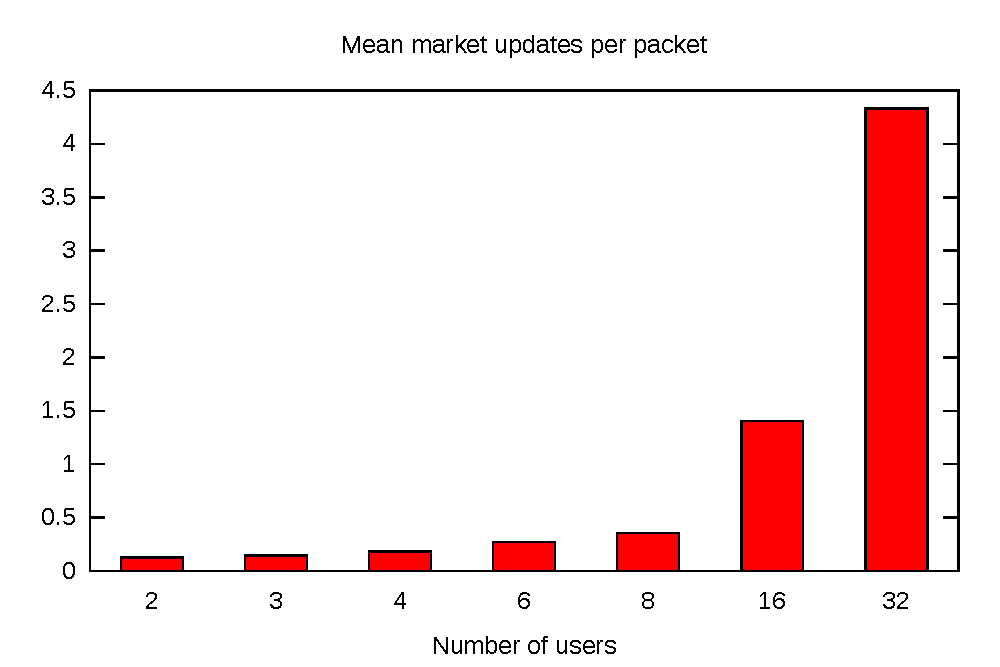
\includegraphics[width=\columnwidth]{plots/num_market_updates.pdf}
\caption{Mean number of sets of slot purchases made by flow completion time bots in simulation.}
\label{f:num_market_updates}
\end{figure}

Another problem with the simple market is that it can take a long time to converge on a solution where no user wants to buy more slots. In simulation, flow completion time user bots would buy back and forth from each other many times, making small price adjustments throughout.  
Figure~\ref{f:num_market_updates} shows the number times a user bought a set of packets on the market, or market updates, per packet sent in the simulations from in Figure~\ref{f:delay_over_srtf}.
More contention between slots increased the number of market updates required.

%TODO improve below sentence
The problems we encountered with the simple market led us to our current design:
\subsection{Multiresolution Market Design}

TODO

\begin{figure*}
\renewcommand{\arraystretch}{2}
\begin{tabular}[height=3in]{|*{8}{p{\slotwidth}|}}
\hline
\multicolumn{8}{|c|}{}\\
\hline
\multicolumn{4}{|c|}{} &\multicolumn{4}{c|}{} \\
\hline
\multicolumn{2}{|c|}{} &\multicolumn{2}{c|}{} &\multicolumn{2}{c|}{} &\multicolumn{2}{c|}{}\\
\hline
Time: 0 & Time: 1 & Time: 2 & Time: 3 & Time: 4 & Time: 5 & Time: 6 & Time: 7 \\
\{(A, \$2.01)\} & \{(A, \$2.01)\} & \{(B, )\} & \{(B, )\} & \{(ISP, \$1)\} & \{(ISP, \$1)\} & \{(C, \$10)\} & \{(ISP, \$1)\} \\
\hline
\end{tabular}
\caption{Multiresolution market order book.}
\label{f:multiresolution _market}
\end{figure*}
